\documentclass[a4paper,12pt]{article}

\usepackage[left=2.5cm, right=2.5cm, top=3cm, bottom=3cm]{geometry}
\usepackage[spanish]{babel}
\usepackage{graphicx}

\begin{document}
    
	\title{"Precios al descubierto: el lado oculto detrás de los alarmantes precios"}
	\author{Marian Aguilar Tavier}
	\date{Julio, 2023}
	\maketitle
	
	\newpage
	\begin{abstract}
		Cuando salimos a las calles, muchas veces nos quedamos impresionados con los grandes cambios que ha experimentado nuestro país en los últimos años. Entre ellos, es imposible pasar por alto el aumento de los precios de los productos, y por esta razón solemos preguntarnos por qué si existen productos que pertenecen a una misma categoría, los precios entre ellos varían considerablemente y no encontramos una explicación adecuada para esto.
		Es por ello que se ha realizado este estudio para determinar si existen o no factores que influyan en el precio de los productos y cómo se evidencian estas características particulares en su precio. El  análisis está centrado en la cerveza, el ron, el whisky, el vodka y la cebolla en Habana del Este, municipio capitalino de gran extensión.
		
		El análisis fue posible mediante la utilización de Python de conjunto con la biblotecas Pandas, Matplotlib y Seaborn.
		A lo largo del desarrollo de informe comprabaremos además que factores como el país de procedencia, el porcentaje de alcohol, el color de la bebida(en el caso de la cerveza), el material del envase tienen una gran influencia sobre el precio del producto.
		Sin embargo, también nos percataremos que no en todos los productos las diferencias en sus características influyen enormemente en el precio, pues en el caso de la cebolla, por ejemplo, casi no existe diferencia en el precio si analizamos el producto por color o por la forma en la que se adquiere(siempre y cuando no sea en ristras).
	\end{abstract}
    \newpage
    
	\tableofcontents
    \newpage
	\section{Introducción}
	Cuba, es un país que a lo largo de los años se ha caracterizado por tener un pueblo el cual siempre estará dispuesto a luchar y vencer ante cualquier tipo de adversidad. Sin embargo, no es menos cierto que en los últimos años el país ha estado atravesando una gran crisis económica que ha dado lugar no solo a que exista una menor disponibilidad de todos aquellos artículos y alimentos que contribuyen al bienestar de la población cubana. La escasez ha traído, además como consecuencia directa, que los precios de los productos a los que el cubano debe acceder día a día hayan sufrido alarmantes variaciones, generalmente desfavorables para el bolsillo del trabajador y del cubano en general.
	Por la importancia que tiene la variación de los precios para el día a día del cubano y para la economía en general, a través de la realización de este proyecto, podremos analizar el comportamiento de algunos de estos productos, algunos de ellos imprescindibles en el hogar como es el caso de la cebolla, así como otros que, aunque son hasta cierto punto dañinos para la salud, contribuyen a que el cubano disfrute y pase un momento agradable al lado de los seres que más quiere. El estudio se basa en el análisis del comportamiento de los precios de una serie de productos, en este caso la cebolla, la cerveza y otro tipo de bebidas alcohólicas(ron, whisky y vodka), con la finalidad de no solo averiguar cuál es el precio promedio de cada producto, sino también de investigar si existen o no factores externos que influyan en la variación de los mismos.
	Este informe está dividido en varias secciones: Introducción, Cerveza, Whisky, Vodka, Ron, Cebolla y Conclusiones.
	
		\newpage
		\subsection{Proceso de captura, extracción y manipulación de datos}
			\subsubsection{Procesaminto de datos}
			Para la realización de este proyecto, se realizó un recorrido por varios sitios del municipio capitalino Habana del Este, específicamente por Cojímar, el Reparto Camilo Cienfuegos, Alamar, Guanabo y el Reparto Antonio Guiteras. En estos lugares se visitaron
			una serie de cafeterías, y todos aquellos lugares a los que la población acude para comprar
			ciertos artículos, pero no se consume en ellos. En el caso de los productos agrícolas como
			la cebolla, se visitaron varios agros. La recopilaci´on de datos se baso en la captura de
			los precios de los productos mediante fotos y se utilizaron los metadatos del m´ovil para
			corroborar la localizacion de los mismos.
			\subsubsection{Extracción y manipulación de los datos}
			Luego de obtener todas las imágenes correspondientes a los precios de los productos
			sometidos a nuestro estudio, comenzamos a procesar los datos a través de la creación
			de una base da datos mediante un archivo en formato .json que nos permite tener un
			mayor control y una mayor organización sobre nuestros datos. Cada producto se analizó
			atendiendo a una serie de categorías, en el caso de la cerveza se analizó la misma con
			respecto a la marca, su localización, la capacidad del envase, el porcentaje de alcohol,
			el precio de la misma, el país de procedencia, su color, el tipo de envase en la que se
			encontraba. El resto de las bebidas alcohólicas en este caso el ron, el whisky y el vodka
			se analizaron atendiendo a las mismas categorías: la marca, el precio de cada producto,
			el material en el que se envasó el producto, su localización, el país de procedencia, el
			porcentaje de alcohol y la capacidad de su envase.
		
			Para manipular este gran volumen de información, utilizamos Python, el cual nos
			permite importar nuestra base de datos (en este caso un archivo en formato .json) con
			su módulo json. La manipulación de los datos fue llevada a cabo mediante la biblioteca
			Pandas, donde cada producto analizado tiene su propio dataframe con la información correspondiente a ese producto. Pandas nos permitió cargar y transformar los conjuntos de
			datos de manera eficiente, aplicar operaciones de filtrado y selección y calcular estadísticas descriptivas. Otras bibliotecas como Matplotlib y Seaborn fueron utilizadas para la
			vizualización de nuestros resultados.
	\newpage
	\section{Cerveza}
		\subsection{Programación empleada}
	     En este caso, utilizamos el dataframe correspondiente al diccionario cerveza de nuestro json. Luego, fuimos analizando el producto en cada categoría para lo cual filtramos las distintas columnas de nuestro dataframe. De esta forma utilizamos varias funciones de Pandas como value.counts() para determinar la disponibilidad de cada marca de cerveza, la función sort.values() para poder establecer un orden de las cervezas más vendidas a las menos vendidas, así como la función .mean para determinar el precio promedio de una cerveza. Otras funciones como groupby, nos permitieron asociar dos columnas de nuestro dataframe, que, unido a la función mean de pandas nos permitió calcular el precio promedio por marca de cerveza. Este mismo procedimiento fue utilizado para determinar que países se consideran que presentan las marcas de cerveza más caras y cuáles las más baratas. En el análisis de la cerveza atendiendo al color de la misma se incorporó toda la información correspondiente a esta columna de nuestro dataframe a una lista vacía y a través de la función .count se pudo establecer la disponibilidad de la cerveza clara con respecto a la disponibilidad de la cerveza oscura. Luego mediante la creación de una función que calcula el porcentaje se pudo establecer qué porcentaje representan las cervezas claras en relación con las cervezas oscuras. Un procedimiento similar fue seguido a la hora de determinar el precio promedio de la cerveza según su color y el tipo de envase, para lo que se filtraron las columnas correspondientes a la categoría específica (ya sea color o tipo de envase) y el precio y se calculó el promedio teniendo en cuenta el color o el tipo de envase de la cerveza. Para analizar la disponibilidad de las marcas nacionales, usando la función isin se filtraron los datos que solo tenían a Cuba como país de procedencia, y de forma similar a como se realizó con el resto de los países se determinó la disponibilidad de cada marca. Para determinar cómo se encuentra distribuida la cerveza atendiendo al envase, se implementó la función len en la columna del dataframe correspondiente a este dato, tanto en el caso de las cervezas embotelladas como en el caso de las cervezas enlatadas. De esta forma fue posible determinar cuál es el tipo de envase predominante. La función .mode fue utilizada para determinar las cerveza más importada en Cuba, para lo cual se filtraron los datos de tal forma que solo aparecieran las cervezas cuyo país de procedencia no fuera Cuba mediante la función isin, luego de negar nuestro dataframe. También se implementó esta función a la hora de indagar el porcentaje de alcohol y la capacidad más común que se puede encontrar en una cerveza en estos sitios. Para determinar el precio promedio de una cerveza según su capacidad se empleó un procedimiento similar, se filtró el data frame atendiendo a la capacidad del envase y se calculó el promedio de los precio de cada capacidad usando la función .mean(). En el caso de la visualización de los resultados obtenidos a raíz de nuestro análisis se empleó Seaborn y Matplotlib, cuyos gráficos en este caso son todos de barra. En el caso de Seaborn a la hora de elaborar los gráficos se modificaron varias opciones como el color de las barras, la orientación de las mismas.
		\subsection{Resultados del análisis}
		Con un simple vistazo a la categoría correspondiente al país del que proviene nuestro producto nos percatamos de que la lista es bastante variada. Entonces surge una pregunta bastante interesante: ¿Cuál es el país que más exporta cerveza hacia Cuba? De la manipulación y el análisis de los datos anteriores se comprueba que el país que más importa cerveza en Cuba es España, seguido muy de cerca por Países Bajos, mientras que otros países como China y Polonia se encuentran entre los país con menos exportaciones en el municipio.
		
		\begin{figure}[h]
			\centering
			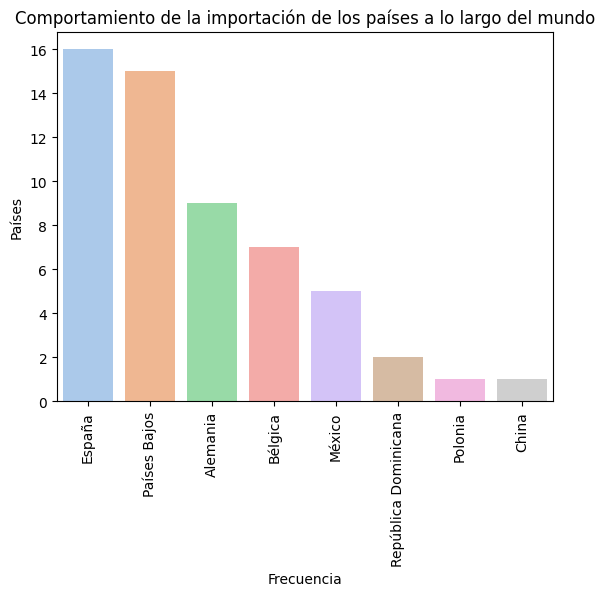
\includegraphics[width=10cm]{export.png}
			\label{fig:Comportamiento de la exportación de cerveza por países}
		\end{figure}
		Si analizamos ahora si existe alguna relación entre el país que más exporta cerveza con el país que más variedades de cervezas exporta, nos percatamos de que España además de ser el país que más se destaca en la exportación, es el que más variedades provee en La Habana del Este con 7 marcas distintas, en segundo lugar se encuentra Países bajos con 5 marcas de cerveza. En último lugar con respecto a las variedades de cerveza se encuentran nuevamente China, Polonia y República Dominicana.
		
		\begin{figure}[h]
			\centering
			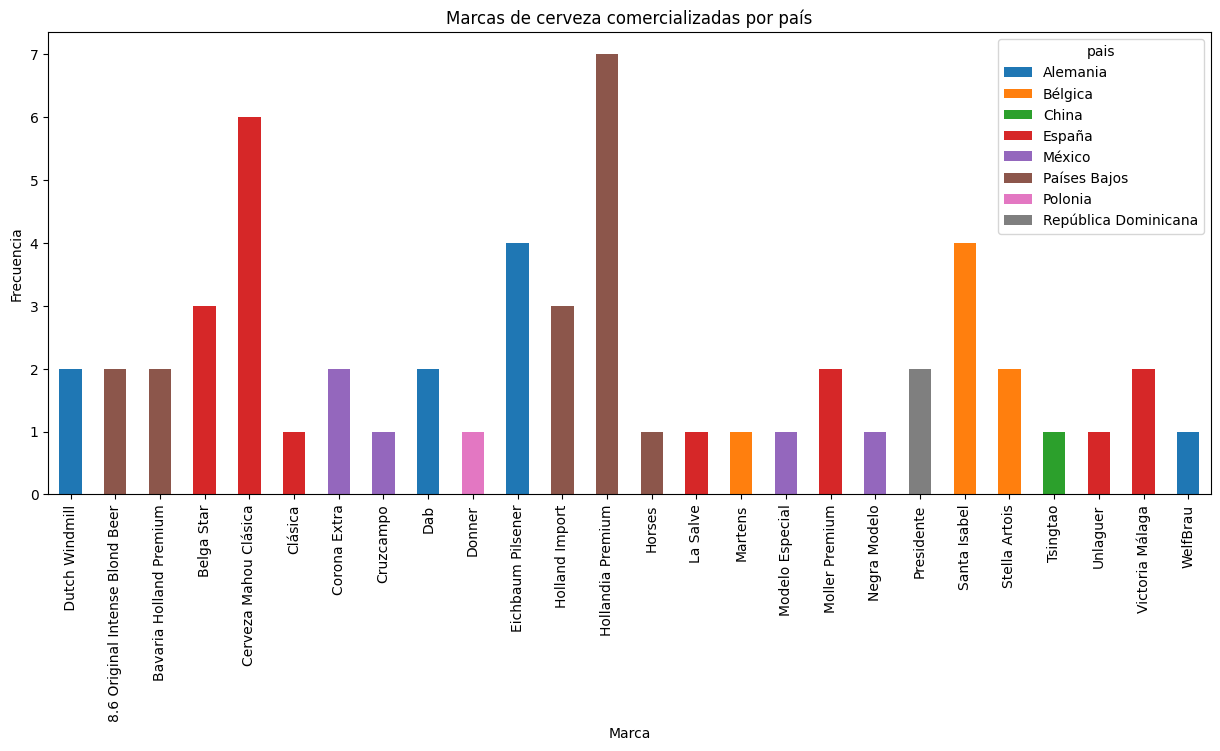
\includegraphics[width=10cm]{country beer.png}
			\label{fig:Variedades de cerveza por país}
		\end{figure}
		¿Qué ocurre si consideramos ahora este producto teniendo en cuenta su precio por marca? Pues en este caso se aprecia que la cerveza más cara es la cerveza WelfBrau, seguida de la Cristal, la Negra Modelo, la Bucanero y la Cristal Extra, por lo que se observa que, aunque existe una gran variedad de cervezas importadas las marcas nacionales están en el top de las cervezas más caras dentro de estos lugares. De la misma forma las cervezas más económicas que se pueden consumir en esta localidad son la cerveza Clásica, la cerveza Mahou Clásica, la Shekels y la Presidente. Luego se aprecia además, que las cervezas españolas se encuentran en las últimas posiciones de nuestro ranking atendiendo a su precio, por lo que además de ser las que presentan mayor disponibilidad, son de las más económicas del mercado.
		
		\begin{figure}[h]
			\centering
			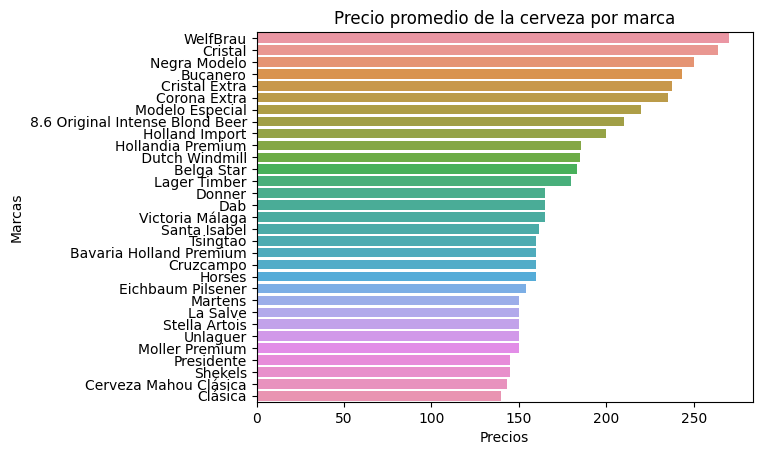
\includegraphics[width=10cm]{price beer.png}
			\label{fig:precio promedio por marca de cerveza}
		\end{figure}
		
		Si observamos la relación existente entre el precio de la cerveza y el país del cual pro viene, apreciamos que el país con las cervezas más económicas es República Dominicana, que unido con Alemania, Bélgica, China y España encabeza el top de las 5 cervezas más económicas en el municipio.
		
		\begin{figure}[h]
			\centering
			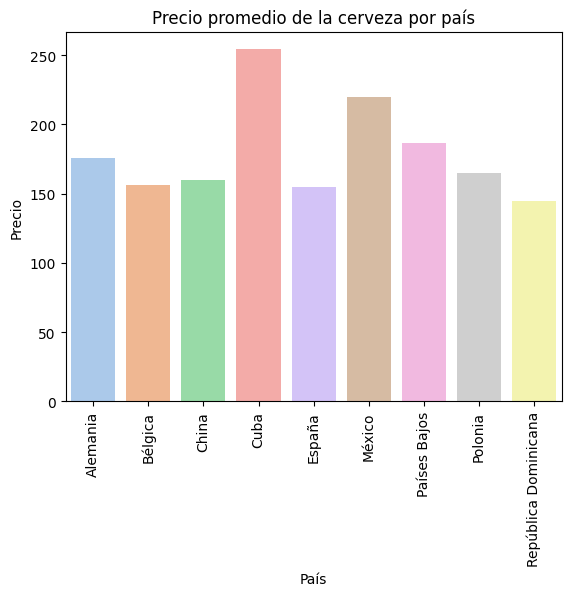
\includegraphics[width=10cm]{price country.png}
			\label{fig:relacion precio-país de la cerveza}
		\end{figure}
		
		Luego de analizar el precio promedio por marca de cerveza y su comportamiento con respecto al país del cual proviene, podemos afirmar que en Habana del Este una cerveza tiene un precio promedio de 191 CUP y la cerveza más importada es la Holland Import. En cuanto a la disponibilidad de la cerveza según el color de esta, se observa que el consumo de las cervezas clara es mucho mayor al consumo de las cervezas oscuras ya que, el 82.05\% representa a las cervezas claras, mientras que las cervezas oscuras representan solo el 14.10\%. Teniendo en cuenta el precio de las mismas a pesar de que las cervezas oscuras presentan una menor disponibilidad, se pueden encontrar a precios mucho más económicos que las cervezas claras, pues el precio promedio de una cerveza clara es de 207 CUP, mientras que el de la cerveza oscura es 188 CUP aproximadamente.
		
		\begin{figure}[h]
			\centering
			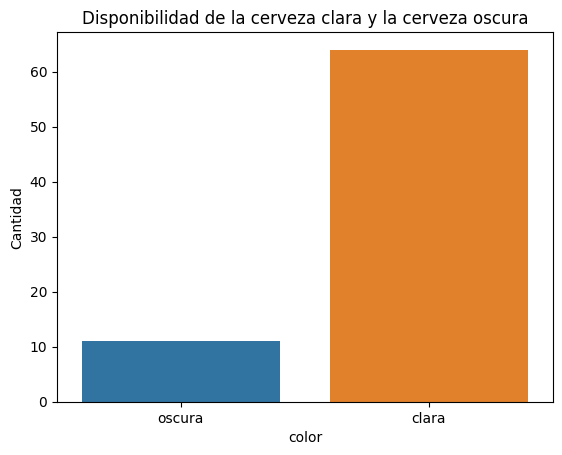
\includegraphics[width=10cm]{dark and light.png}
			\label{fig:cerveza según su color}
		\end{figure}
		
		Realicemos ahora un análisis más profundo, pero esta vez con respecto a las marcas nacionales, donde, como resultado de nuestro análisis, as cervezas que se encontraron fueron la Cristal, la Bucanero y la Cristal Extra. De estas, la cerveza con mayor disponibilidad es la Cristal, seguida de la Cristal Extra y la menos accesible es la cerveza Bucanero.
		
		\begin{figure}[h]
			\centering
			\includegraphics[width=10cm]{cuban beer  amount.png}
			\label{fig:Disponibilidad de las marcas nacionales}
		\end{figure}
		
		El precio de la cerveza teniendo en cuenta su disponibilidad, no provoca en este caso una diferencia muy notable pues, la cerveza cristal además de ser la más disponible es la más cara, seguida de la Bucanero y en último lugar la Cristal Extra.
		
		\begin{figure}[h]
			\centering
			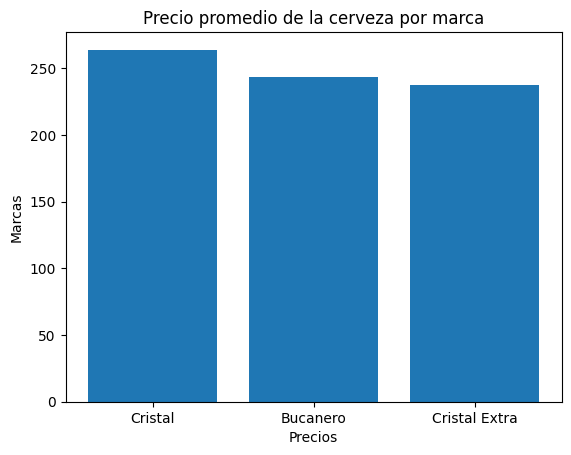
\includegraphics[width=10cm]{cuban beer price.png}
			\label{fig:Precio de las marcas nacionales}
		\end{figure}
		
		Analizando este producto según el envase en el que se encuentra, encontramos cervezas en botellas y en latas, y aunque podemos encontrar este producto de ambas formas, cabe destacar que predominan las cervezas enlatadas por encima de las embotelladas, representando las primeras el 85.88\% del total de cervezas. Mientras que solo el 12.82\% corresponde a las latas de cerveza embotelladas. Pero ¿a qué se debe que el número de envases de lata sea superior al número de cervezas en botella? Si analizamos las características de cada uno, considerando que las cervezas de lata se fabrican normalmente de aluminio, se enfrían más rápido, lo cual representa una ventaja para el dueño de una cafetería con abundante flujo de clientes. Es más conveniente que estas sean de lata ya que en el caso de Guanabo por ejemplo, sitio de gran interés para todos aquellos extranjeros que deciden pasar sus vacaciones en las cálidas aguas del Caribe, resulta realmente importante adquirir el producto bien frío, situación que aunque también puede ser posible con las botellas de cristal, se tarda más tiempo en enfriarse. Por lo que la disponibilidad de la cerveza según el tipo de envase favorece a los vendedores del producto. En cuanto al porcentaje de alcohol más común que se encuentra en una cerveza en este municipio es de 4.9\%. Con el análisis del tipo de envase del producto, nos percatamos de que la cantidad de ml de alcohol puede influir o no en el precio de la cerveza. En general una cerveza en Habana del Este, independientemente de su tipo de envase tiene una capacidad de 330 ml. Si analizamos la diferencia de precio entre las cervezas en lata y de botella con la misma cantidad de ml, nos percatamos de que la diferencia de precio es mínima, ya que el precio de una cerveza en lata oscila entre los 162 CUP y el de la cerveza en botella en 160 CUP.
		
	\section{Ron}
		\subsection{Programación empleada}
		En el caso de este producto, se extrajo la información procedente del diccionario ron de nuestro json, solo que esta vez se filtraron los datos del dataframe que correspondieran con este tipo de bebida. Luego a partir de nuestro nuevo dataframe filtrado, se utilizaron varias funciones empleadas anteriormente para obtener un buen análisis de nuestros datos. Una vez más se empleó la función .mean de Pandas para cal cular el precio promedio del ron tanto de forma general, como a la hora de calcular el precio promedio por marca, con ayuda de groupby. Para poder analizar los rones nacionales, filtramos la nuestro dataframe utilizando isin para todos aquellos rones cuyo país de procedencia es Cuba. Para investigar la disponibilidad de cada marca, empleamos nuevamente las funciones value.count() y sort.values() para ordenarlas de la más disponible a la menos disponible. Este resultado se muestra mediante un gráfico de barras en Seaborn. Luego los resultados del cálculo del precio promedio de cada ron, se visualizó mediante un gráfico de barras horizontales en Seaborn. El filtrado también se utilizó a la hora de determinar el precio promedio del ron según el material del envase, para lo que se calculó el promedio del precio de los rones embotellados en plástico y los rones embotellados en cristal, información que aparece en una de las columnas del dataframe que corresponde al material del envase. La función .mode se empleó para determinar cuál es el porcentaje de alcohol más común que se encuentra en una botella de ron. Para determinar los rones con mayor y con menor porcentaje de alcohol se utilizó nuevamente la función sort.values() para ordenar los porcentajes de los rones de mayor a menor. Para calcular el precio promedio del ron según su capacidad, se crearon dos nuevos DataFrames filtrados, atendiendo a la columna correspondiente a la capacidad en ml. Luego se calculó el precio promedio de cada uno de estos DataFrames.
		\subsection{Resultados del análisis}
		La implementación de todas las funciones mencionadas anteriormente nos permitieron arribar a los siguientes resultados: Al acercarnos a los productos nacionales(dado que en este caso la mayoría de los rones son cubanos), nos encontramos no solo con una amplia variedad de marcas, sino también que los mismos difieren en cuanto a su tipo de envase, ya que los podemos encontrar tanto en botellas de plástico, como en botellas de cristal y lo mismo sucede con si capacidad que va desde 700 ml hasta 1000 ml. El porcentaje de alcohol también sufre algunas modificaciones teniendo en cuenta la marca. Pero ¿influirán todos estos factores en su precio? De forma general una botella de ron en Habana del Este tiene un precio promedio de 2161 CUP independientemente de todas las características mencionadas anteriormente. En cuanto a la disponibilidad del producto si bien es cierto, que existe varias marcas de ron, no presentan la misma disponibilidad y en este caso, el ron que más es posible encontrar en el Havana Club Añejo Especial, seguido del Havana Club Reserva. Mientras que otros rones como el Galeón, el Havana Club 7 Años y el Ron Santiago de Cuba 8 Años tienen una menor disponibilidad.
		
		\begin{figure}[h]
			\centering
			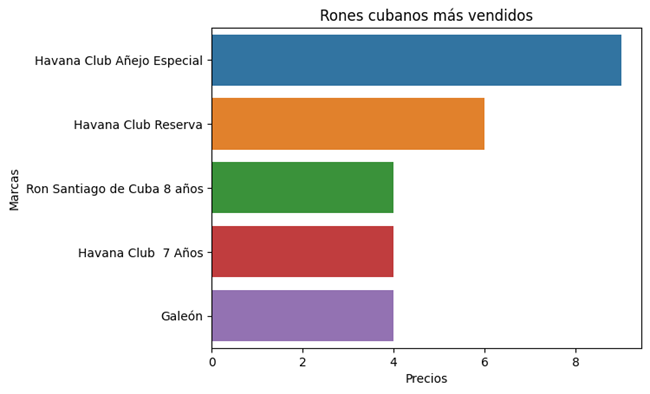
\includegraphics[width=12cm]{cuban rum.png}
			\label{fig:Disponibilidad de los rones cubanos}
		\end{figure}
		
		Al investigar el precio promedio de cada marca de ron, nos percatamos de que no se observa el mismo patrón que en el caso de las cervezas cubanas donde la disponibilidad era directamente proporcional al precio de la cerveza. En este caso los rones que presentan mayor disponibilidad se encuentran en el rango intermedio de precios. Mientras que los rones más caros son el Havana Club Selección de Maestros, el Ron Santiago de Cuba 11 Años y el Pacto Navío. Al calcular el precio promedio de los rones envasados en botellas de plástico en relación con los rones envasados en botellas de cristal nos percatamos de que la diferencia de precios entre estos dos tipos de envases es relevante ya que mientras el precio promedio de un ron envasado en plástico es de 728 CUP y el precio promedio de una botella de ron de cristal es de 2428.75 CUP. Sin embargo, solamente conociendo este dato referente al material del envase no es suficiente para generalizar sobre el precio promedio de ambos rones, ya que también depende de la cantidad de ml del recipiente y su porcentaje de alcohol. Si analizamos por otro lado, el porcentaje de alcohol en el caso del ron, una botella de ron en Habana del Este suele encontrarse con un porcentaje de alcohol de 40\% sin embargo, aunque este es el porcentaje de alcohol más común, hay rones que se encuentran por encima y otros por debajo de este porcentaje. Veamos entonces cómo se comporta el porcentaje de alcohol por marca de ron:
		
		\begin{figure}[h]
			\centering
			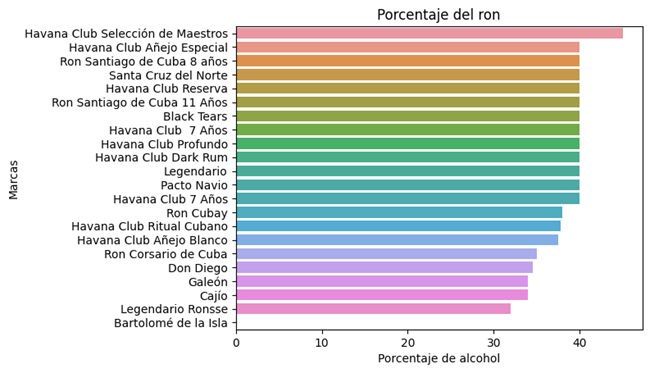
\includegraphics[width=10cm]{alcohol rum.png}
			\label{fig:Porcentaje de alcohol de los rones por marca}
		\end{figure}
		
		\begin{figure}[h]
			\centering
			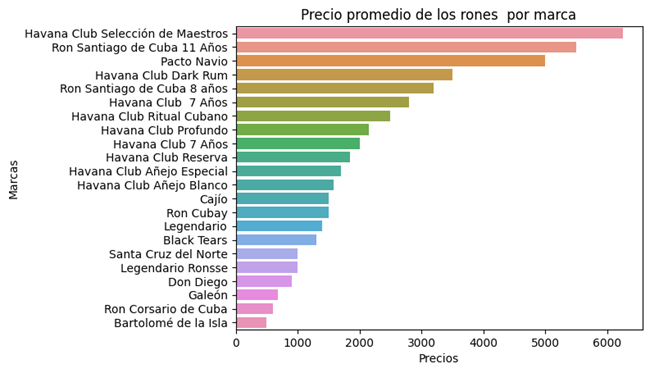
\includegraphics[width=11cm]{rum prices.png}
			\label{fig:Precio promedio del ron por marca}
		\end{figure}
		
		Al analizar el precio promedio del ron según la capacidad que estos presentan, la diferencia es notable. Mientras que el precio promedio de una botella de ron de 750 mililitros es de 1100 CUP, el precio promedio de una botella de 1000 ml es de 1517 CUP aproximadamente.
		
	\section{Whisky}
		\subsection{Programación empleada}
		
		En el caso del Whisky el código empleado es muy similar al del ron. Se empleó la función .mean para determinar el precio promedio de una botella de whisky. La función .mode fue utilizada para averiguar cuál es el país que más exporta whisky en Cuba, así como para conocer la marca más importada.
		
		\subsection{Resultado del análisis}
		El whisky es un producto que, al igual que el ron se destaca por tener una serie de características pueden influir o no en su precio, sin embargo, el precio promedio de una botella de whisky es de aproximadamente 2801 CUP. En cuanto a las marcas de whisky la que más se exporta en este municipio es el whisky Chanceler, seguido del Old Partner y el Chanceler Edición Especial. Se observa además que Brasil, que es el país que representa a whisky más importado no coincide con el país que más importa whisky, ya que este lugar está ocupado por Escocia, en segundo lugar Brasil y en tercer lugar España.
		
			\begin{figure}[h]
			\centering
			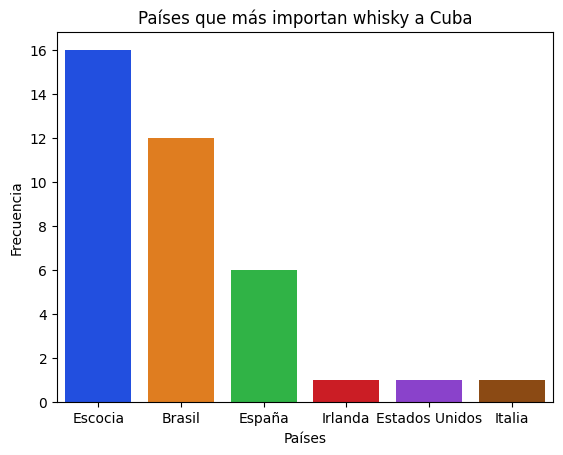
\includegraphics[width=12cm]{whisky export.png}
			\label{fig:Comportamiento del whisky por países}
		\end{figure}
		
	\section{Vodka}
		\subsection{Programación empleada}
		La metodología empleada para el análisis de los datos relacionados con esta bebida es similar a las dos anteriores. En este caso empleamos la función .mean para calcular el precio promedio del vodka luego de filtrar nuestro DataFrame. La moda para determinar cuál era el vodka más importado y el porcentaje de alcohol más común que se encuentra en una botella de Vodka. Luego también se empleó la función sort.values para ordenar los whiskys desde el que presenta mayor porcentaje de alcohol, al que tiene menor porcentaje de alcohol.
		
		\subsection{Resultados del análisis}
		En el caso de este producto, muy consumido también por la población cubana, se observa una disminución en cuanto al precio en comparación de los dos productos anteriores, luego en Habana del Este el precio promedio de una botella de vodka es de 1964 CUP. A pesar de la existencia de una amplia variedad de marcas de este, muchas de ellas provenientes de Rusia, el más importado en este caso es el de la marca Tabarish, el cual también es un vodka ruso. Al igual que el whisky, el vodka coincide en cuanto al porcentaje de alcohol más común que se encuentra en una botella, siendo en este caso de 40\% de alcohol. Y aunque es el porcentaje más común a pesar de ser además el más alto que se puede encontrar en el municipio, también existen otros que se encuentra por debajo de este porcentaje, por lo que resultan un poco menos perjudiciales para la salud. En esta categoría se encuentra el Vodka Krilof Black, cuyo porcentaje de alcohol es de un 20\%, sin embargo cabe destacar que aunque este porcentaje está por debajo del promedio, continúa siendo una gran amenaza para la salud humana, por lo que se debe ingerir con moderación al igual que el resto de las bebidas alcohólicas antes mencionadas. De forma general analicemos los precios de los tres productos anteriores:
		
			\begin{figure}[h]
			\centering
			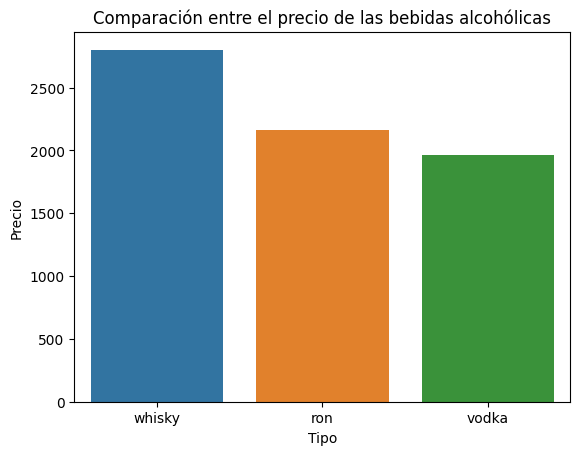
\includegraphics[width=12cm]{comparation.png}
			\label{fig:Comparación de precios}
		\end{figure}
		
	En este caso observamos que de las tres bebidas el whisky tiene un precio más elevado
	que el ron, mientras que el vodka es la bebida más barata de las tres.
	
	\section{Cebolla}
		\subsection{Programación empleada}
		Para el análisis de los datos relacionados con este productos se creó un dataframe que contuviera los datos referentes al diccionario cebolla de nuestro archivo en formato json. El mismo se analizó atendiendo a su precio, su color, la forma en la que se puede adquirir, ya sea en pote, en libra o en ristra, así como su localización. Para calcular el precio promedio de la cebolla atendiendo a su color, crearon dos nuevos dataframes filtrados en relación al color de la cebolla y luego a través de la función .mean() se calculó el promedio de los precios. Luego este resultado fue ilustrado median te un gráfico de barras utilizando Seaborn. Se utilizaron las funciones value.counts() y sort.values() para analizar la disponibilidad de la cebolla según a la categoría en la que se vendía, ya fuera en libras, en pote o por unidad. Luego estos resultados se ilustraron en un gráfico de barras.
		\subsection{Resultados del análisis}
		Si bien la cebolla es un producto que no guarda mucha relación con los productos mencionados anteriormente, constituye un alimento imprescindible en las cocinas cubanas, no solo por el simple hecho de reportar múltiples beneficios para la salud, sino también porque forma parte de nuestro increíble sazón cubano el cual es reconocido a nivel internacional. Realizar un estudio sobre el precio de este producto en particular, resulta bastante complejo ya que no en todas las ocasiones este producto se encuentra disponible. Al analizar el precio de la cebolla según su color, los resultados arrojan a que la diferencia de precio atendiendo al color de la cebolla es muy pequeña. Mientras que el precio promedio de la cebolla blanca es de aproximadamente 164 CUP, el de la cebolla morada es de 154 CUP.
		
		\begin{figure}[h]
			\centering
			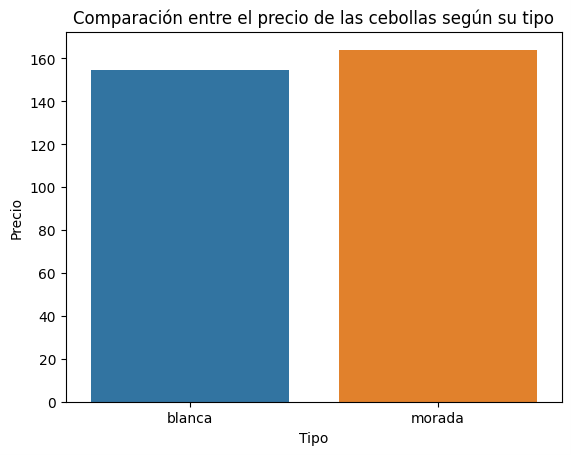
\includegraphics[width=10cm]{onion.png}
			\label{fig:Comparación entre el precio de la cebolla}
		\end{figure}
		
	
	
	\newpage
	\section{Conclusiones}
	Con el desarrollo de este proyecto investigativo de Ciencia de Datos, pudimos comprobar que efectivamente, existen varios factores que influyen en el precio de los productos analizados. No se trata de un precio descabellado sin ninguna referencia como tal, sino que, aunque algunos factores tienen una mayor influencia que otros, todos contribuyen a la hora de establecer el precio final. En cuanto al proceso para la obtención de nuestros resultados hemos comprobado que Pandas, resultó ser de gran ayuda, ya que a través del filtrado de la información y a partir de sus diferentes funciones, fue posible obtener los resultados de nuestro análisis. Si bien es cierto que los precios de los productos son de por sí bastante elevados, a lo largo de este proyecto investigativo hemos podido comprobar que el factor precio se ve influenciado por una serie de elementos, que a la vez varían en dependencia del producto. En el caso de las bebidas alcohólicas (incluyendo a la cerveza) en general se han observado ciertos patrones en cuanto al precio dependiendo del país del que procede el producto, el porcentaje de alcohol, la cantidad de mililitros del envase, el color de la bebida, el tipo, y en el material en el cual se envasa. Al analizar la cebolla también se han observado variaciones en su precio teniendo en cuenta el color de esta y la escasa disponibilidad si se tiene en cuenta las diferentes formas en las que se pueden encontrar las mismas. Es importante mencionar que nuestro estudio de los precios está comprendido entre los meses de abril y mayo del año 2023. Por lo que puede ser utilizado posteriormente para el análisis de los precios de estos productos en años posteriores para así analizar su variación a lo largo del tiempo.
	
\end{document}

